\underline{Photodiode}

The final part of this experiment deals with inserting a photodiode into the circuit. It should be noted that a phototransistor is used instead of a photodiode since a  phototransistor has similar characteristics as a photodiode when light is illuminated onto it, even being more sensitive to light. For this particular part, the phototransistor has a wide depletion layer that helps more excited electrons be exposed to light. When light is illuminated onto the phototransistor, the transistor absorbs many photons and produces a lot of power. Photons at a high frequency excite electrons from the valence band to the conduction band since their energy level is higher than the bandgap energy. The phototransistor is to be regarded in three cases (reverse bias, zero bias, and forward bias). When electrons jump from the valence band to conduction band, the electric field in the region with a shortage of electrons cause the electrons to move in a reverse-biased direction. The reverse bias current is driven by the excited electrons, which as a result supply the load with power. The second case for this phototransistor is being zero biased. The flow of current out of the transistor is restricted and a voltage builds up, which leads to some amount of power generation. For both cases of reverse bias and zero bias, the voltage drop over the transistor increases as light shines on the phototransistor, therefore these two biases generate the most power compared to the forward bias. The power generated and power efficiency from both of the biases is very similar because of the widened depletion layer. The third and final case is when the diode is in forward bias. When the diode is in forward bias, the depletion layer of the diode is decreased thus not much power being generated. Therefore, the voltage drop over the phototransistor is the same when the light is both off and on. The only source of power comes from the supply voltage. \\



\underline{10}
When working with solar cells (pn-junction) the best case to collect energy of light is by shining light on a photodiode. When the light is illuminated on the diode, the photons are absorbed and more power is produced by converting light energy into electrical energy. This only occurs if the diode is in reverse bias, so there is an increase in effect of the electric field which contributes to current. Reverse bias helps the holes depart from the valence band and helps the electrons depart from the conduction band while also enhancing the potential. This results in carriers being excited and going towards either the cathode or anode electrodes. Electron-hole pairs are formed when light is illuminated onto a diode which results in reverse current. If the diode is in forward bias there will be almost negligible current due to the current flowing in only one direction. This occurs when the p-type carries are made more positive while the n-type carriers are made more negative. The charge carriers move very slowly and this leads to the solar cell being less effective. If a PIN diode is used, it is even better since there is an intrinsic semiconductor layer between the n-type layer and p-type layer that will help excited electrons be exposed to light. This concludes that power efficiency is at its best when the photodiode is in reverse bias since the output power divided by input power is much larger than forward bias due to no voltage change.\\
\begin{table}
	\centering
	\begin{tabular}{| c | c | c | c |}\hline
		& V\textsubscript{in}=-5V & V\textsubscript{in}=0 & V\textsubscript{in}=5V \\\hline
		Without Flashlight & -0.01 & 0.075 & 0.82\\\hline
		With Flashlight & 0.50 & 0.52 & 0.82 \\\hline
	\end{tabular}
\label{Voltage over Photodiode}
\ref{photodiode_table}
\end{table}

\begin{figure}[h!]
	\centering
	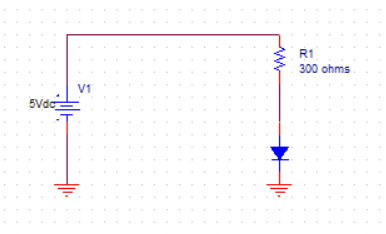
\includegraphics{CircuitSchematic.PNG}
	\caption{Experiment 4 Circuit}
	\label{fig:Circuit_Pic}
\end{figure}

\section{References}
\scriptsize{
	\begin{enumerate}
		\item \url{https://www.stanley-components.com/data/technical_note/TN014_e.pdf}
		\item \url{https://romikoderbynew.com/2011/02/25/reverse-bias-in-solar-cells/}
	\end{enumerate}
}

